\section{Discrete Event Simulation}\label{sec:discrete_event_simulation}

Discrete Event Simulation (DES) is a method for modelling the behaviour of
real-world systems in which the system is made up of discrete events, each of
which has a certain duration~\cite{DESstewart}.
It can be used to understand complex situations in order to make predictions
and thus provide improvements~\cite{VinceGeraintBook}.
The three main approaches to building DES models are the activity scanning
approach, the event scheduling approach and the process interaction
approach~\cite{DESapproaches}.
Under the scope of this study only the event scheduling approach is considered.
This section describes the DES model used to
represent the queueing network of Section~\ref{sec:queueing_section}.

In order to use DES on the queueing network shown in
Figure~\ref{fig:diagram_of_queueing_system} an equivalent queueing network must
be constructed.
The current queueing network is a two-node queueing system that accepts two
types of individuals, where type 1 individuals arrive at node 1 and
type 2 individuals arrive at node 2.
The modification that is required revolves around the mechanisms of node 2.
Node 2 is defined as a non-service node where there is only a queueing
space for individuals to wait there until they are allowed to node 1.
From an implementation perspective there is an equivalent system that can be
used where instead of a node with no service and queueing capacity \(M\), there
are \(M\) servers each serving with a service rate of \(0\) and no queueing
capacity, as shown in Figure~\ref{fig:equivalent_diagram_of_queueing_system}.

\begin{figure}[H]
    \centering
    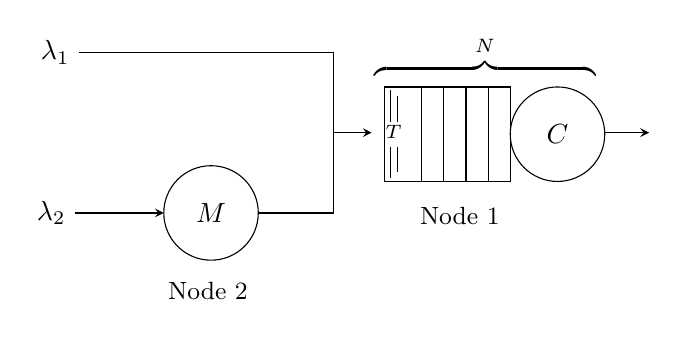
\begin{tikzpicture}[>=stealth, scale=0.8],

    % the circle in Queue 1
    \draw (2.25cm, -0.75cm) circle [radius=0.75cm] node {\(M\)};

    % The label below Queue 1 -> Node 2
    \node[anchor=north] at (2.2cm, -1.7cm) {\small{Node 2}};

    % the rectangle in Queue 2
    \draw (5, 1.25) -- ++(2cm, 0) -- ++(0, -1.5cm) -- ++(-2cm, 0);
    % the vertical lines in Queue 2
    \foreach \i in {1,...,4, 5.7}
    \draw (7cm-\i*10pt,1.25) -- +(0,-1.5cm);
    % The two vertical lines at the start of Queue 2
    \draw (7cm-54pt,1.2) -- +(0,-0.5cm);
    \draw (7cm-54pt,0.3) -- +(0,-0.5cm);
    \draw (7cm-51pt,1.1) -- +(0,-0.4cm);
    \draw (7cm-51pt,0.3) -- +(0,-0.4cm);

    % The label between the lines for T
    \node[anchor=north] at (5.15, 0.79 cm) {\scriptsize \( T \)};

    % The label above Queue 2 -> N
    \node[anchor=north] at (6.6cm, 2.2cm) {\(
        \overbrace{\qquad \qquad \qquad \qquad}^{N}
    \)};
    % The label below Queue 2 -> Node 1
    \node[anchor=north] at (6.2cm, -0.5cm) {\small{Node 1}};

    % the circle in Queue 2
    \draw (7.75,0.5) circle [radius=0.75cm] node {\(C\)};

    % Arrow line from Queue 2 outside
    \draw[->] (8.5,0.525) -- +(20pt,0);

    % Line from lambda_2 to Queue 1
    \draw[<-] (1.5,-0.75) -- +(-40pt,0) node[left] {\( \lambda_2 \)};
    % First line (horizontal) after Queue 1
    \draw[-] (3,-0.75) -- +(34pt,0);
    % Second line (vertical) after Queue 1
    \draw (4.2, 0.525) -- (4.2, -0.75);

    % First line (horizontal) from lambda_1
    \draw (4.2, 1.8) -- +(-115pt,0) node[left] {\( \lambda_1 \)};
    % Second line (vertical) from lambda_1
    \draw (4.2, 1.8) -- (4.2, 0.525);
    % Arrow line to Queue 2
    \draw[->] (4.2, 0.525) -- (4.8, 0.525);
\end{tikzpicture}

    \caption{An equivalent model to the one described in
    Figure~\ref{fig:diagram_of_queueing_system}. The difference between the two
    diagrams is the formulation of node 2. The original diagram uses
    a node with no servers and a queueing capacity of \(M\) while this one uses
    \(M\) servers with no queueing capacity.}
    \label{fig:equivalent_diagram_of_queueing_system}
\end{figure}
    

The arrival times for both nodes are exponentially distributed with
mean \(\lambda_1\) and \(\lambda_2\) corresponding to type 1 and type 2
individuals respectively.
Node 1 has an exponentially distributed service time with rate \(\mu\),
a total of \(C\) servers and a queueing capacity of \(N - C\) (making the
overall capacity \(N\)). 
Node 2 has a deterministic service time of \(0\), a total of \(M\)
servers and a queueing capacity of \(0\).
Note here that, similar to Figure \ref{fig:diagram_of_queueing_system},
parameters \(N\) and \(M\) are used to approximate the real world system 
and in fact can be taken to be infinite in the DES.
Finally the routing parameter is defined as an array that probabilistically
routes individuals from all nodes to all other nodes.
For this particular system the routing parameter needs only to route individuals
from node 2 to node 1.

\begin{equation}
    \text{routing parameter} = \left[
    \begin{array}{cc}
        0 & 1 \\
        0 & 0
    \end{array}
    \right]
\end{equation}


\subsection{Implementation}
The python library \texttt{ciw}~\cite{ciwpython, ciwarticle}
was used to implement the DES model.
The library treats queues as distinct nodes in the network where each node has
an arrival distribution, a service distribution, a number of available servers
and a queue capacity.

The following code can be used to generate a queueing network with two
queues and two types of individuals, where type 1 individuals arrive at node
1 with an arrival rate of \texttt{lambda\_1} and type 2
individuals arrive at node 2 with an arrival rate of
\texttt{lambda\_2}.
Node 2 has a deterministic fixed service rate of
\texttt{0} (since there is no service involved in the buffer
centre) and node 1 has an exponential service rate of
\texttt{mu}.

\begin{lstlisting}[
    style=pystyle,
    caption={Using the \texttt{ciw} library to create a queueing network with
    two queues and two types of individuals and the particular structure
    defined in Figure~\ref{fig:equivalent_diagram_of_queueing_system}.},
    label={lst:create_initial_queueing_network},
]
>>> import ciw
>>> lambda_1 = 1.0
>>> lambda_2 = 2.0
>>> mu = 0.5
>>> num_of_servers = 3
>>> system_capacity = 10
>>> buffer_capacity = 5
>>> model = ciw.create_network(
...     arrival_distributions=[
...         ciw.dists.Exponential(lambda_2),
...         ciw.dists.Exponential(lambda_1)
...     ],
...     service_distributions=[
...         ciw.dists.Deterministic(0), ciw.dists.Exponential(mu)
...     ],
...     routing=[
...         [0.0, 1.0],
...         [0.0, 0.0]
...     ],
...     number_of_servers=[buffer_capacity, num_of_servers],
...     queue_capacities=[0, system_capacity - num_of_servers],
... )

\end{lstlisting}

As described earlier in Section~\ref{sec:queueing_section} and as shown in
Figure~\ref{fig:diagram_of_queueing_system}, type 1 individuals arrive at
node 1 and exit the system after their service finishes, but type 2 individuals
arrive at node 2 and then proceed to node 1 after leaving node 2.
This logic is implemented in the queueing network using the
\texttt{routing} parameter that consists of the routing
probabilities between different nodes.
For the current implementation the routing matrix is a \(2 \times 2\) array
that routes individuals from node 2 to node 1 with a probability of
\(1.0\).
Furthermore, the server availability for nodes 1 and 2 are set to
the \texttt{num\_of\_servers} and
\texttt{buffer\_capacity} respectively and the queue capacities
are set to \texttt{system\_capacity - num\_of\_servers} and \texttt{0}.
Note that for node 2 queue capacity is set to 0 and its
number of servers is set to the buffer capacity.
From \texttt{ciw}'s data records perspective this made more
sense since individuals are recorded as blocked this way.
If the queue capacity was non-zero, individuals could also have a waiting time
but no waiting should take place in node 2, only blockage.


\subsection{Custom node class}
Another specific feature of the particular model is that type 2 individuals
need to stay blocked in node 2 whenever the number of individuals in node 1
reaches a certain threshold \(T\).
As opposed to the rest of the model, this portion of the queueing network
requires more effort to build.
\texttt{Ciw} allows users to get more custom behaviour by
creating their own node class that inherits from the original one.
By inheriting the original \texttt{ciw.Node} the general
behaviour of all nodes can be altered.
Note that node ids are assigned in the order they are created so in the
\texttt{ciw} implementation node 2 is assigned id 1 and node 1
is assigned id 2.


\begin{lstlisting}[
    style=pystyle,
    caption={Function that contains the custom node class that blocks
    individuals to node 1 when the number of individuals in node 2 exceeds
    the threshold.},
    label={lst:build_custom_node},
]
>>> import numpy as np
>>> def build_custom_node(threshold=float("inf")):
...     """
...     Build a custom node to replace the default ciw.Node. Inherits from
...     the original ciw.Node class and replaces methods
...     release_blocked_individual and finish_service.
...     The methods are modified in such a way that all individuals that
...     are in the buffer space (node 1) stay blocked as long as the
...     number of individuals in the service area node (node 2) exceeds the
...     threshold.
...
...     Parameters
...     ----------
...     threshold : int, optional
...         The capacity threshold to be used by the method
...     Returns
...     -------
...     class
...         A custom node class that inherits from ciw.Node
...     """
...
...     class CustomNode(ciw.Node):
...         """
...         Overrides the default release_blocked_individual and
...         finish_service methods of the ciw.Node class
...         """
...
...         def __init__(self, id_, simulation):
...             """
...             Initializes the node with the given id and simulation using
...             the initialisation of ciw's Node object with the addition of
...             the threshold parameter.
...             """
...             super().__init__(id_, simulation)
...             self.simulation.threshold = threshold
...
...         def release_blocked_individual(self):
...             """
...             Releases an individual who becomes unblocked when
...             another individual is released:
...             - check if individual in node 2 and should stay blocked
...                 i.e. if the number of individuals in that
...                      node > threshold
...             - check if anyone is blocked by this node
...             - find the individual who has been blocked the longest
...             - remove that individual from blocked queue
...             - check if that individual had their service interrupted
...             - release that individual from their node
...             """
...             continue_blockage = (
...                 self.number_of_individuals >= threshold
...                 and self.id_number == 2
...             )
...             if (
...                 self.len_blocked_queue > 0
...                 and self.number_of_individuals < self.node_capacity
...                 and not continue_blockage
...             ):
...                 receiving_node = (
...                     self.simulation.nodes[self.blocked_queue[0][0]]
...                 )
...                 individual_to_receive_index = [
...                     ind.id_number
...                     for ind in receiving_node.all_individuals
...                 ].index(self.blocked_queue[0][1])
...                 individual_to_receive = (
...                     receiving_node.all_individuals[
...                         individual_to_receive_index
...                     ]
...                 )
...                 self.blocked_queue.pop(0)
...                 self.len_blocked_queue -= 1
...                 if individual_to_receive.interrupted:
...                     individual_to_receive.interrupted = False
...                     receiving_node.interrupted_individuals.remove(
...                         individual_to_receive
...                     )
...                     receiving_node.number_interrupted_individuals -= 1
...                 receiving_node.release(individual_to_receive_index, self)
...
...         def finish_service(self):
...             """
...             The next individual finishes service:
...             - finds the individual to finish service
...             - check if they need to change class
...             - find their next node
...             - release the individual if there is capacity at destination,
...                 otherwise cause blockage
...             - Note that blockage also occurs when we are at node 1 and
...                 the number of individuals on node 2 are more than the
...                 'threshold'
...             """
...             (
...                 next_individual,
...                 next_individual_index
...             ) = self.find_next_individual()
...             self.change_customer_class(next_individual)
...             next_node = self.next_node(next_individual)
...             next_individual.destination = next_node.id_number
...             if not np.isinf(self.c):
...                 next_individual.server.next_end_service_date=float("Inf")
...             blockage = (
...                 next_node.number_of_individuals >= threshold
...                 and self.id_number == 1
...             )
...             if (
...                 next_node.number_of_individuals < next_node.node_capacity
...             ) and not blockage:
...                 self.release(next_individual_index, next_node)
...             else:
...                 self.block_individual(next_individual, next_node)
...
...     return CustomNode

\end{lstlisting}

The class \texttt{CustomNode} inherits from \texttt{ciw}'s
\texttt{Node} class and changes two of the methods
(\texttt{release\_blocked\_individual} and
\texttt{finish\_service}) so that the additional logic of the
threshold is incorporated.
In the \texttt{release\_blocked\_individual} method an
additional check is added before releasing a potentially blocked individual from
node 2 to node 1.
This essentially checks whether the id number of the node is 2 and
the number of individuals in it are more than or equal to the
\texttt{threshold} so that it can accept a blocked individual.
Similarly \texttt{finish\_service} is called once an individual
finishes their service.
The additional check that was added checks whether the id of the node is 1 and
the number of individuals in the next node (i.e. node 1) is more than the
threshold, which would result in blockage.
Finally, the simulation object can be created and simulated for a specific
\texttt{threshold} and \texttt{runtime} by running:

\begin{lstlisting}[
    style=pystyle,
    caption={Building and simulating the network model using the custom node},
    label={lst:simulating_with_custom_node},
]
>>> threshold = 4
>>> runtime = 1000
>>> custom_node = build_custom_node(threshold)
>>> ciw.seed(0)
>>> simulation = ciw.Simulation(model, node_class=custom_node)
>>> simulation.simulate_until_max_time(runtime)

\end{lstlisting}


\subsection{Performance Measures}

Having run the simulation using \texttt{ciw} all necessary
performance measures can be calculated.
Calculating all performance measure that are related to the duration of time is
not too difficult.
The code snippet in~\ref{lst:des_performance_measures} gets all waiting times,
service times and blocking times for all individuals that have passed through
the model.

\begin{lstlisting}[
    style=pystyle,
    caption={Function that extracts performance measures from the simulation
    records},
    label={lst:des_performance_measures},
]
>>> def extract_times_from_records(simulation_records, warm_up_time):
...     """Get the required times (waiting, service, blocking) out of ciw's
...     records where all individuals are treated the same way. This function
...     can't distinguish between class 1 and class 2 individuals. It returns
...     the aggregated waiting time, service times BUT only blocking times of
...     class 2 individuals.
...     """
...     waiting_times = [
...         r.waiting_time
...         for r in simulation_records
...         if r.arrival_date > warm_up_time and r.node == 2
...     ]
...     serving_times = [
...         r.service_time
...         for r in simulation_records
...         if r.arrival_date > warm_up_time and r.node == 2
...     ]
...     blocking_times = [
...         r.time_blocked
...         for r in simulation_records
...         if r.arrival_date > warm_up_time and r.node == 1
...     ]
...     return waiting_times, serving_times, blocking_times

\end{lstlisting}

Using the earlier variable \texttt{simulation}, the waiting
times, service times and blocking times can be extracted from the simulation
records.

\begin{lstlisting}[
    style=pystyle,
    caption={Using the function defined in~\ref{lst:des_performance_measures}},
    label={lst:des_performance_measures_example},
]
>>> warm_up_time = 100
>>> all_records = simulation.get_all_records()
>>> waiting_times, serving_times, blocking_times = extract_times_from_records(
...     all_records, warm_up_time
... )
>>> np.mean(waiting_times), np.mean(serving_times), np.mean(blocking_times)
(1.7038750111337655, 2.041619227158985, 8.227702587974997)

\end{lstlisting}

The performance measures discussed so far are the ones that are related to the
amount of time that individuals spend in the system.
Some additional performance measures that could be of interest are the
ones that are related to the number of individuals, such as the mean number of
individuals in the system, the mean number of individuals in Node 1 and the
mean number of individuals in Node 2.
These metrics can also by calculated using an additional functionality of
\texttt{ciw}.
There is an additional argument that can be passed to the
\texttt{ciw.Simulation} object called \texttt{tracker} where it makes the
simulation object track the state of the system throughout the simulation.
Thus, at the end of the simulation, the probability distribution of the number
of individuals in each node can be extracted.
Section~\ref{sec:queueing_performance_measures} gives a more detailed
explanation of how to calculate these performance measures using only the
state probabilities of the system.
